\chapterimage{golden_gate.jpg}
\chapter{Layer 3: Internet(work) communication}\label{sec:layer3}

\begin{minipage}{0.4\linewidth}
\begin{center}
\begin{bytefield}{16}
\bitbox{16}{Layer 7: Application} \\
\bitbox{16}{Layer 4: Transport} \\
\bitbox{16}{\color{color1} Layer 3: Internet} \\
\bitbox{16}{Layer 2: Network (LAN)} \\
\bitbox{16}{Layer 1: Physical} \\
\end{bytefield}
\end{center}
\end{minipage}
\begin{minipage}{0.6\linewidth}
\begin{center}
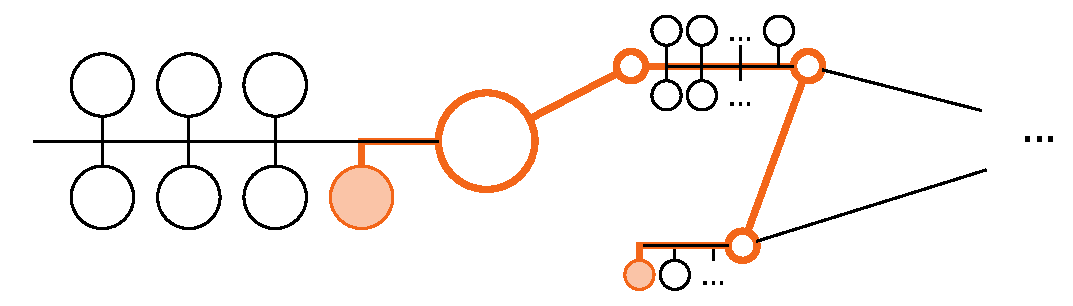
\includegraphics[width=\linewidth]{network_layer3.pdf}
\end{center}
\end{minipage}

\vspace{-0.75cm}

\subsection*{Capabilities}

The \conceptRef{IP}{Internet Protocol (IP)} allows exchanging \concept{datagrams} 
(Layer~3 \conceptRef{PDU}{PDUs}) between devices from different \conceptRef{LAN}{LANs},
with potentially different Layer~2 technologies (\eg \concept{Ethernet} and \concept{Wi-Fi}).

Its addressing system identifies devices globally and makes it possible to 
\conceptRef{routing}{route} datagrams anywhere we need.

Since \conceptRef{datagram}{datagrams} may travel through networks not controlled 
by neither the source nor the destination, datagrams may be lost, reordered and duplicated.

Layer~3 does not provide mechanisms to deal with this; upper layers must implement
protection mechanisms when required 
(\eg, to implement \concept{TCP}'s \conceptRef{stream}{data streams}).


\vspace{-0.25cm}
\subsection*{Protocols}

Version~4 of \concept{IP} is \textit{the} protocol used in Layer~3, \ie,
it is common to virtually all communications in the Internet as we know it today.
% 
For many years, the Internet has been struggling to transition towards \concept{IPv6}, 
but the process is not complex and only \concept{IPv4} provides global coverage.

\begin{remark}
In this guide, \concept{IP} means \concept{IPv4} by default.
\end{remark}


The following protocols encapsulate their \conceptRef{PDU}{PDUs} in the payload of IP 
\conceptRef{datagram}{datagrams}:\\[-0.6cm]
\begin{itemize}
\item Transport Control Protocol (\concept{TCP}) 
\item User Datagram Protocol (\concept{UDP})
\item Internet Control Message Protocol (\concept{ICMP})
\end{itemize}

\concept{IPv4} delegates in the \concept{ARP} protocol the translation of known IP addresses 
into MAC addresses within each LAN.

\subsection*{Addressing}

\concept{IPv4} addresses are $32$~bit long. They are most often presented to humans in
the \concept{quad decimal} format, \eg, \otherBase{142.250.201.67}. 

Most IP addresses are \conceptRef{public IP}{public} and unique across the Internet, \ie, the previous IP 
has the same meaning worldwide and identifies a single device.

Many addresses are \conceptRef{private IP}{private}, have special meanings
and cannot be used for routing datagrams through the Internet, including:
\begin{itemize}
\item The \otherBase{127.*.*.*} and \otherBase{0.*.*.*} blocks cannot leave the local computer.
\item The \otherBase{172.*.*.*} and \otherBase{192.168.*.*} cannot leave the \concept{LAN}.
\item \otherBase{255.255.255.255} is reserved for the \concept{local IP broadcast} IP 
(used by \concept{DHCP}).
\end{itemize}

\begin{remark}
The same private address can be used by multiple devices if they belong to different LANs.
\end{remark}

\begin{exercise}\ \\[-0.5cm]
\begin{itemize}
\item How many different \concept{IPv4} addresses are there (including reserved and private)? 
\item Are they sufficient now and in the future?
\item Is it problematic that an address like \otherBase{192.168.0.1} can be used by thousands
  of computers in the Internet right now?
\end{itemize}
\end{exercise}


\subsection*{Practical aspects}

\section{IP addresses, netmasks and CIDR format}\label{sec:layer3:cidr}
also division

\section{ARP}
\begin{remark}
The \concept{ARP} protocol does \textit{not} use IP headers.
\end{remark}

\section{Routing}

\section{ICMP}

\section{Fragmentation}


% - talk about the problem of having different networks, different technologoies (ARPA, XEROX
% - longest prefix matching for routing tables
% - first draft: 8-bit network addresses (a bit off!)
